\chapter{Especiação e macroevolução}\label{ch:b2:speciation}

Numa pequena ilha das Galápagos, em 1982, alguns tentilhões-terrestres
de bico grande chegaram de uma ilha vizinha e ficaram. Durante vinte
anos, competiram com o tentilhão-terrestre-médio residente pelas
\omterm{def:b2:angiosperm-reproduction:seed}{sementes} grandes que ambos preferiam; então veio uma seca, as \omterm{def:b2:angiosperm-reproduction:seed}{sementes}
grandes escassearam, e os residentes de bico maior --- os que competiam
mais diretamente com os recém-chegados --- morreram de fome. Em uma
geração, os bicos dos residentes tinham diminuído, de modo mensurável,
afastando-se dos bicos dos invasores. Duas espécies que se encontraram
foram empurradas para longe uma da outra. Este capítulo trata da
formação das espécies: o que é uma espécie e o que a mantém distinta,
como uma população se torna duas, a competição que afasta as populações
quando elas se encontram, e a visão de longo prazo do registro fóssil,
onde o mesmo processo, repetido mais de cem milhões de vezes, dá a
árvore da vida.

\section{O que é uma espécie}

\begin{definition}[Espécie]\label{def:b2:speciation:species}
\index{conceito de espécie}\index{conceito biológico de espécie}\index{isolamento reprodutivo}
Segundo o \emph{conceito biológico de espécie}, uma espécie é um grupo
de populações cujos membros podem se cruzar entre si e produzir
descendentes férteis, e que estão \emph{reprodutivamente isoladas} de
outros grupos desse tipo: o que une uma espécie é o \omterm{prop:b2:population-genetics:migration}{fluxo gênico}, e o
que separa as espécies é sua ausência. O conceito funciona para os
organismos sexuados de uma época e de um lugar, que são a maior parte do
que um biólogo encontra; ele falha para as linhagens assexuadas (que são
nomeadas por semelhança), para os fósseis (que não podem ser cruzados) e
para os muitos casos em que a fronteira é permeável --- carvalhos e
salgueiros que hibridizam entre espécies, patos cujas espécies se cruzam
em cativeiro, espécies em anel nas quais as populações vizinhas se cruzam
ao longo de todo o contorno de uma barreira até que as extremidades se
encontram e não se cruzam. Outros conceitos preenchem as lacunas: a
espécie \emph{morfológica} (um agrupamento de formas semelhantes), a
\emph{filogenética} (a menor linhagem diagnosticável), a
\emph{ecológica} (uma linhagem que ocupa seu próprio nicho). Nenhum está
errado; cada um mede algo real, e a especiação é o processo pelo qual
eles passam a concordar.
\end{definition}

\begin{proposition}[Mecanismos de isolamento]\label{prop:b2:speciation:isolation}
\index{mecanismo de isolamento}\index{isolamento pré-zigótico}\index{isolamento pós-zigótico}\index{regra de Haldane}
O \omterm{prop:b2:population-genetics:migration}{fluxo gênico} entre duas populações é interrompido por barreiras que
agem antes ou depois da fecundação. \emph{Pré-zigóticas}: as populações
vivem em hábitats diferentes ou se reproduzem em estações diferentes
(isolamento temporal: duas rãs que coaxam em meses diferentes); elas não
reconhecem a corte uma da outra (comportamental: os cantos dos grilos,
os códigos luminosos dos vaga-lumes, as danças dos patos); suas
genitálias ou suas \omterm{def:b2:angiosperm-reproduction:flower}{flores} não se encaixam (mecânico); seus gametas não
se fundem (gamético: as proteínas de ligação ao espermatozoide dos
ouriços-do-mar, os \omterm{def:b2:meiosis-heredity:vocabulary}{alelos}
$S$ do \cref{ch:b2:angiosperm-reproduction}).
\emph{Pós-zigóticas}: o híbrido morre como embrião, ou vive mas é
estéril (a mula; os híbridos de duas espécies de \emph{Drosophila}), ou
é fértil mas seus próprios descendentes não o são (colapso híbrido).
\emph{\omterm{prop:b2:speciation:isolation}{Regra de Haldane}}: quando só um sexo de um híbrido é estéril ou
inviável, é o sexo com dois \omterm{prop:b2:meiosis-heredity:sexlinked}{cromossomos sexuais} diferentes --- o macho
nos mamíferos e nas moscas, a fêmea nas aves e nas borboletas ---,
porque as incompatibilidades recessivas do X ficam expostas nele. As
barreiras pré-zigóticas são mais baratas, pois nenhum gameta é
desperdiçado, e a seleção as constrói onde as pós-zigóticas já existem.
\end{proposition}

\begin{theorem}[Por que os híbridos falham: o modelo de dois lócus]\label{thm:b2:speciation:dm}
\index{incompatibilidade de Dobzhansky--Muller}
Duas populações partem do \omterm{def:b2:meiosis-heredity:vocabulary}{genótipo} $aabb$. Numa, $a$ é substituído por
$A$; na outra, $b$ por $B$; cada substituição é neutra ou favorável em
seu próprio contexto genético, de modo que nenhuma população jamais
passa por um estado de menor \omterm{def:b2:population-genetics:fitness}{aptidão}. Mas $A$ e $B$ nunca foram testados
juntos e, se a combinação for incompatível --- se a proteína produzida
por $A$ não conseguir funcionar com a proteína produzida por $B$ ---, o
híbrido $AaBb$ é inapto. O \omterm{def:b2:speciation:species}{isolamento reprodutivo} surge assim como um
subproduto da divergência, sem nenhum vale atravessado e sem seleção
para o isolamento em si; e, como cada nova substituição numa linhagem
pode ser incompatível com cada substituição já fixada na outra, o
número de incompatibilidades possíveis cresce com o
\emph{quadrado} do número de substituições --- o isolamento
\emph{cresce como uma bola de neve} com o tempo.
\end{theorem}
\begin{proof}
Com $n$ substituições em cada linhagem, cada um dos $n$ novos \omterm{def:b2:meiosis-heredity:vocabulary}{alelos} de
uma linhagem pode ser incompatível com cada um dos $n$ da outra:
$n^{2}$ pares, cada um incompatível com alguma probabilidade
$\varepsilon$, de modo que o número esperado de incompatibilidades é
$\varepsilon n^{2}$, e $n$ cresce com o tempo decorrido desde a
separação. O híbrido é o único \omterm{def:b2:meiosis-heredity:vocabulary}{genótipo} em que os dois conjuntos se
encontram.
\end{proof}
\begin{proof}[Evidências]
Coyne e Orr (1989, 1997) reuniram centenas de pares de espécies de
\emph{Drosophila} de distância genética conhecida (uma medida do tempo
desde a divergência) e mediram seu \omterm{prop:b2:speciation:isolation}{isolamento pré-zigótico} e
pós-zigótico: ambos aumentam com a distância, o isolamento é praticamente
completo a uma distância que corresponde a alguns milhões de anos, e os
pares que vivem na mesma região mostram, a uma dada distância, um
\omterm{prop:b2:speciation:isolation}{isolamento pré-zigótico} mais forte que os pares que não vivem juntos ---
a assinatura do reforço. Os genes de incompatibilidade foram desde então
identificados um a um, e o número encontrado entre duas espécies de fato
cresce mais depressa que linearmente com sua divergência.
\end{proof}

\begin{omfigure}
\begin{tikzpicture}[every node/.style={font=\scriptsize}, >=stealth]
  \node[draw, rounded corners, fill=omExo!25] (anc) at (0,0) {ancestral $aabb$};
  \node[draw, rounded corners, fill=omDef!15] (p1) at (-2.6,-1.8) {população 1: $AAbb$};
  \node[draw, rounded corners, fill=omThm!15] (p2) at (2.6,-1.8) {população 2: $aaBB$};
  \node[draw, rounded corners, fill=gray!25, align=center] (hyb) at (0,-3.6) {híbrido $AaBb$:\\$A$ e $B$ se encontram pela primeira vez\\--- incompatíveis, inapto};
  \draw[->, thick] (anc) -- (p1) node[midway, left, align=right] {$a \to A$ fixado,\\apto em seu contexto};
  \draw[->, thick] (anc) -- (p2) node[midway, right, align=left] {$b \to B$ fixado,\\apto em seu contexto};
  \draw[->, thick] (p1) -- (hyb); \draw[->, thick] (p2) -- (hyb);
  \node[anchor=west, align=left, text width=4.6cm] at (4.6,-0.4) {nenhuma população atravessou um vale; o isolamento é um subproduto, e o número desses pares cresce como $n^{2}$};
\end{tikzpicture}

{\small O modelo de dois lócus do fracasso dos híbridos. Cada população
fixa uma mudança que funciona em seu próprio contexto; o híbrido é o
primeiro \omterm{def:b2:meiosis-heredity:vocabulary}{genótipo} a combinar as duas.}
\end{omfigure}

\section{Como uma espécie se torna duas}

\begin{proposition}[Modos de especiação]\label{prop:b2:speciation:modes}
\index{especiação alopátrica}\index{especiação simpátrica}\index{especiação parapátrica}\index{efeito fundador}
A especiação \emph{alopátrica} começa com uma barreira geográfica: uma
área de distribuição dividida por uma montanha que se ergue, um mar que
seca ou um novo rio (\emph{vicariância}), ou alguns colonos levados a
uma ilha (\emph{peripátrica}, com o \omterm{prop:b2:speciation:modes}{efeito fundador} e a deriva do
\cref{ch:b2:population-genetics} de quebra). Isoladas do \omterm{prop:b2:population-genetics:migration}{fluxo gênico},
as duas populações divergem pela seleção em ambientes diferentes, pela
deriva e por suas \omterm{def:b2:genome-diversification:mutation}{mutações} próprias, até que as incompatibilidades se
acumulem; se voltarem a se encontrar, já não se fundem. É o modo mais
comum, e o padrão de espécies-irmãs em lados opostos de cada istmo,
cadeia de montanhas e estreito é o seu registro. A especiação
\emph{simpátrica} ocorre sem barreira: de uma só vez, por \omterm{def:b2:genome-diversification:polyploidy}{poliploidia}
(\cref{ch:b2:genome-diversification}) --- um terço das espécies de
plantas surgiu assim; ou por seleção disruptiva com cruzamento
preferencial, quando uma população explora dois recursos e os
indivíduos se acasalam sobre o recurso que utilizam (a mosca-da-maçã,
que passou do espinheiro para a macieira nos anos 1860 e hoje se acasala
sobre seu hospedeiro; os ciclídeos de um lago de cratera). A especiação
\emph{parapátrica} ocorre ao longo de um gradiente ambiental, onde uma
população se adapta às duas extremidades e uma \omterm{prop:b2:speciation:reinforcement}{zona híbrida} se forma no
meio. Em todos os modos, a receita é a mesma: reduzir o \omterm{prop:b2:population-genetics:migration}{fluxo gênico},
deixar a divergência se acumular e deixar que os subprodutos da
divergência se tornem barreiras.
\end{proposition}

\begin{omfigure}
\resizebox{\linewidth}{!}{%
\begin{tikzpicture}[every node/.style={font=\scriptsize}, >=stealth]
  \foreach \x/\lab in {0/{alopátrica:\\uma barreira divide a área}, 5.2/{peripátrica:\\alguns fundadores numa ilha}, 10.4/{simpátrica:\\dois hospedeiros,\\acasalamento no hospedeiro}} \node[align=center, anchor=south] at (\x+1.8,3.0) {\lab};
  % allopatric
  \draw[thick, fill=omDef!15] (0.9,1.4) ellipse (0.8 and 0.9);
  \draw[thick, fill=omThm!15] (2.7,1.4) ellipse (0.8 and 0.9);
  \draw[very thick, omExo!70!black] (1.8,0.2) -- (1.8,2.6);
  \node[below] at (1.8,0.1) {montanha, mar, rio};
  % peripatric
  \begin{scope}[xshift=5.2cm]
    \draw[thick, fill=omDef!15] (1.0,1.4) ellipse (1.0 and 0.9);
    \draw[thick, fill=omThm!15] (3.2,1.9) circle (0.35);
    \draw[->, thick, dashed] (2.0,1.6) -- (2.85,1.85);
    \node[below] at (3.2,1.5) {fundadores};
    \node[below] at (1.0,0.4) {continente};
  \end{scope}
  % sympatric
  \begin{scope}[xshift=10.4cm]
    \draw[thick, fill=omExo!15] (1.8,1.4) ellipse (1.7 and 0.9);
    \foreach \p in {(1.0,1.6),(1.3,1.2),(0.8,1.2),(1.2,1.8)} \fill[omDef] \p circle (0.07);
    \foreach \p in {(2.4,1.6),(2.7,1.2),(2.2,1.2),(2.6,1.8)} \fill[omThm] \p circle (0.07);
    \node[omDef, below] at (1.0,0.5) {planta A}; \node[omThm, below] at (2.6,0.5) {planta B};
    \node[below] at (1.8,0.1) {um lugar, dois recursos};
  \end{scope}
\end{tikzpicture}}

{\small Três caminhos para duas espécies: uma barreira através da área
de distribuição, uma população fundadora além dela, ou dois recursos
dentro dela.}
\end{omfigure}

\begin{proposition}[Reforço e zonas híbridas]\label{prop:b2:speciation:reinforcement}
\index{reforço}\index{zona híbrida}\index{clina}
Quando duas populações que divergiram voltam a se encontrar, três coisas
podem acontecer. Se seus híbridos forem tão aptos quanto os pais, elas
se fundem. Se os híbridos forem inaptos, a seleção favorece os
indivíduos que se recusam a cruzar com a outra forma --- os gametas
desperdiçados são o custo --- e o \omterm{prop:b2:speciation:isolation}{isolamento pré-zigótico} se fortalece
onde as duas se sobrepõem (\emph{reforço}), até que se tornem espécies.
Entre esses casos, persiste uma \emph{\omterm{prop:b2:speciation:reinforcement}{zona híbrida}}: uma faixa, muitas
vezes de alguns quilômetros de largura, onde as duas formas se cruzam e
híbridos são produzidos a cada geração, mantida pelo equilíbrio entre a
dispersão para dentro da zona e a seleção contra os híbridos dentro
dela. Através de tal zona, a frequência de cada forma segue uma
\emph{clina}, uma curva em forma de S cuja largura $w$ é fixada pela
distância de dispersão $\sigma$ por geração e pela seleção $s$ contra os
híbridos, $w \approx
\sigma\sqrt{8/s}$: uma zona pode permanecer estreita por milhares de
anos sem que as duas formas jamais se fundam ou se separem por completo.
Os sapos, as gralhas, os camundongos e os gafanhotos da Europa mostram
dezenas delas, a maioria ao longo das linhas onde populações que tinham
se abrigado em refúgios separados durante a última glaciação voltaram a
se encontrar quando o gelo recuou.
\end{proposition}
\begin{proof}[Evidências]
Onde o papa-moscas-preto e o papa-moscas-de-colar se sobrepõem, na
Europa central, os machos de cada espécie têm uma plumagem mais
diferente da do outro do que onde vivem separados, e as fêmeas
discriminam com mais rigor --- o reforço medido no campo. O
sapo-de-barriga-de-fogo e o sapo-de-barriga-amarela se encontram ao longo de uma
zona que atravessa a Polônia, com alguns quilômetros de largura, estável
desde que começou a ser estudada, com a largura da clina prevista a
partir de sua dispersão e da \omterm{def:b2:population-genetics:fitness}{aptidão} reduzida de seus híbridos.
\end{proof}

\begin{omfigure}
\begin{tikzpicture}
\begin{axis}[
  width=0.72\linewidth, height=5.2cm,
  axis x line=bottom, axis y line=left,
  xmin=-30, xmax=30, ymin=0, ymax=1.05,
  xlabel={distância através da zona (km)}, ylabel={frequência da forma A},
  xlabel style={font=\small, at={(axis description cs:0.5,-0.13)}, anchor=north},
  ylabel style={font=\small},
  tick label style={font=\small}, xtick={-20,-10,0,10,20}, ytick={0,0.5,1},
  clip=false,
]
\addplot[very thick, omDef, domain=-30:30, samples=100] {1/(1+exp(x/2.2))};
\draw[dashed, gray] (axis cs:-4.4,0) -- (axis cs:-4.4,1); \draw[dashed, gray] (axis cs:4.4,0) -- (axis cs:4.4,1);
\draw[<->] (axis cs:-4.4,0.08) -- (axis cs:4.4,0.08); \node[font=\scriptsize, anchor=south] at (axis cs:0,0.09) {largura $w$};
\node[font=\scriptsize, anchor=west, align=left] at (axis cs:8,0.75) {$w \approx \sigma\sqrt{8/s}$: dispersão\\$\sigma = \qty{1}{km}$, $s = 0.1$\\dão $w \approx \qty{9}{km}$};
\end{axis}
\end{tikzpicture}

{\small Uma clina através de uma \omterm{prop:b2:speciation:reinforcement}{zona híbrida}: a frequência de uma forma
cai de um a zero ao longo de uma largura fixada pela distância a que os
indivíduos se dispersam e pela inaptidão de seus híbridos.}
\end{omfigure}

\section{Competição, coexistência e deslocamento de caracteres}

\begin{theorem}[Competição de Lotka--Volterra]\label{thm:b2:speciation:lv}
\index{competição de Lotka--Volterra}\index{exclusão competitiva}\index{coexistência}
Duas espécies de crescimento logístico (volume do Ano 1) que competem
por um recurso obedecem a
\[
\frac{\mathrm{d}N_1}{\mathrm{d}t} = r_1 N_1\Bigl(1 - \frac{N_1 + \alpha N_2}{K_1}\Bigr), \qquad
\frac{\mathrm{d}N_2}{\mathrm{d}t} = r_2 N_2\Bigl(1 - \frac{N_2 + \beta N_1}{K_2}\Bigr),
\]
em que $\alpha$ mede o efeito de um indivíduo da espécie 2 sobre a
espécie 1 em unidades de indivíduos da própria espécie 1, e $\beta$ o
inverso. A espécie 1 para de crescer sobre a reta $N_1 + \alpha N_2 =
K_1$ (sua \emph{isóclina}), a espécie 2 sobre $N_2 + \beta N_1 = K_2$, e
o desfecho depende de como as duas retas se cruzam:
\begin{itemize}
  \item $K_1 > \alpha K_2$ e $K_2 < \beta K_1$: a espécie 1 vence
        sempre;
  \item $K_1 < \alpha K_2$ e $K_2 > \beta K_1$: a espécie 2 vence
        sempre;
  \item $K_1 > \alpha K_2$ e $K_2 > \beta K_1$: \emph{coexistência
        estável} em $N_1^{*} = (K_1 - \alpha K_2)/(1 - \alpha\beta)$,
        $N_2^{*} = (K_2 - \beta K_1)/(1 - \alpha\beta)$;
  \item $K_1 < \alpha K_2$ e $K_2 < \beta K_1$: qualquer uma vence,
        conforme a que começar mais numerosa.
\end{itemize}
A coexistência exige $\alpha\beta < 1$, com cada espécie mais contida
pelos de sua própria espécie que pela outra: duas espécies que usam
exatamente o mesmo recurso ($\alpha = \beta = 1$) não podem coexistir
(o \emph{princípio da \omterm{thm:b2:speciation:lv}{exclusão competitiva}}), e quanto mais elas
diferem naquilo que usam, menores são $\alpha$ e $\beta$ e mais
seguramente coexistem.
\end{theorem}
\begin{proof}
Sobre a isóclina da espécie 1, $\mathrm{d}N_1/\mathrm{d}t = 0$; abaixo
dela (em direção à origem) $N_1$ cresce, acima dela $N_1$ diminui; o
mesmo vale para a espécie 2. Cada isóclina é uma reta com interceptos
$K_1$ no eixo $N_1$ e $K_1/\alpha$ no eixo $N_2$ (a da espécie 1),
$K_2/\beta$ e $K_2$ (a da espécie 2). A espécie 1 pode invadir uma
população da espécie 2 em sua capacidade de suporte $K_2$ se seu próprio
crescimento for positivo ali, isto é, se $K_1 > \alpha K_2$; a espécie 2
pode invadir a espécie 1 em $K_1$ se $K_2 > \beta K_1$. Quando cada uma
pode invadir a outra, nenhuma pode ser excluída e as trajetórias
convergem para o cruzamento das isóclinas, encontrado resolvendo as
equações das duas retas; quando só uma pode, ela vence; quando nenhuma
pode, o cruzamento é um ponto de sela e vence a que se estabeleceu
primeiro. A estabilidade do ponto interior decorre do argumento da
invasão: perturbada em direção a qualquer eixo, a espécie mais rara
volta a crescer.
\end{proof}

\begin{omfigure}
\begin{tikzpicture}
\begin{axis}[
  width=0.6\linewidth, height=6cm,
  axis x line=bottom, axis y line=left,
  xmin=0, xmax=1300, ymin=0, ymax=1900,
  xlabel={$N_1$}, ylabel={$N_2$},
  xlabel style={font=\small, at={(axis description cs:0.5,-0.1)}, anchor=north},
  ylabel style={font=\small},
  tick label style={font=\small}, xtick={0,857,1000,1333}, xticklabels={0,$N_1^*$,$K_1$,$K_2/\beta$}, ytick={0,286,800,2000}, yticklabels={0,$N_2^*$,$K_2$,$K_1/\alpha$},
  clip=false,
]
\addplot[very thick, omDef, domain=50:1000, samples=2] {(1000-x)/0.5};
\addplot[very thick, omThm, domain=0:1333, samples=2] {800-0.6*x};
\fill[black] (axis cs:857,286) circle (2.5pt);
\draw[->, thick, gray] (axis cs:150,1750) -- (axis cs:300,1450);
\draw[->, thick, gray] (axis cs:1200,100) -- (axis cs:1000,250);
\draw[->, thick, gray] (axis cs:150,150) -- (axis cs:400,250);
\node[font=\scriptsize, omDef, anchor=west] at (axis cs:700,1000) {isóclina da espécie 1};
\node[font=\scriptsize, omThm, anchor=south west] at (axis cs:130,740) {isóclina da espécie 2};
\node[font=\scriptsize, anchor=south west] at (axis cs:880,320) {coexistência estável};
\end{axis}
\end{tikzpicture}

{\small O plano de fase de dois competidores com $K_1 = 1000$, $K_2 =
800$, $\alpha = 0.5$, $\beta = 0.6$: cada espécie pode invadir a
capacidade de suporte da outra, e as trajetórias convergem para o
cruzamento das isóclinas em $N_1^{*} = 857$, $N_2^{*} = 286$.}
\end{omfigure}

\begin{proposition}[Deslocamento de caracteres]\label{prop:b2:speciation:displacement}
\index{deslocamento de caracteres}\index{nicho}\index{radiação adaptativa}
A competição não é apenas um desfecho ecológico, mas uma força
evolutiva. Onde duas espécies semelhantes se encontram, os indivíduos de
cada uma que mais se parecem com a outra são os que mais sofrem com a
competição, e a seleção afasta as duas no caráter que governa o uso do
recurso --- o tamanho do bico, o tamanho do corpo, a época de floração:
as populações que se sobrepõem diferem mais que as populações que vivem
sozinhas. Esse \emph{\omterm{prop:b2:speciation:displacement}{deslocamento de caracteres}} reduz $\alpha$ e
$\beta$, converte uma disputa por exclusão em coexistência e, repetido
por uma paisagem de oportunidades, produz uma \emph{\omterm{prop:b2:speciation:displacement}{radiação
adaptativa}}: um colono que se torna uma dúzia de espécies, cada uma
ajustada a um recurso --- os tentilhões de Darwin nas Galápagos, os
drepanidíneos do Havaí, os ciclídeos dos lagos africanos (quinhentas
espécies no lago Vitória em menos de quinze mil anos), os lagartos
\textit{Anolis} do Caribe, onde o mesmo conjunto de nichos foi ocupado
pelo mesmo conjunto de formas corporais de modo independente em quatro
ilhas.
\end{proposition}
\begin{proof}[Evidências]
Os Grant registraram todos os tentilhões de Daphne Major durante quarenta
anos. Depois que o tentilhão-terrestre-grande se estabeleceu em 1982, o
bico do tentilhão-terrestre-médio não mudou até a seca de 2004, quando
as \omterm{def:b2:angiosperm-reproduction:seed}{sementes} grandes escassearam e as duas espécies competiram por elas;
os tentilhões médios de bico maior morreram em proporção excessiva, e os
bicos da geração seguinte ficaram menores, numa medida jamais vista num
único passo --- o \omterm{prop:b2:speciation:displacement}{deslocamento de caracteres} previsto pela teoria,
observado enquanto acontecia, com seu diferencial de seleção e sua
herdabilidade medidos. Os bicos desses mesmos tentilhões, comparados
entre ilhas onde vivem sozinhos e ilhas onde se encontram, mostram o
mesmo deslocamento inscrito através do arquipélago.
\end{proof}

\begin{omfigure}
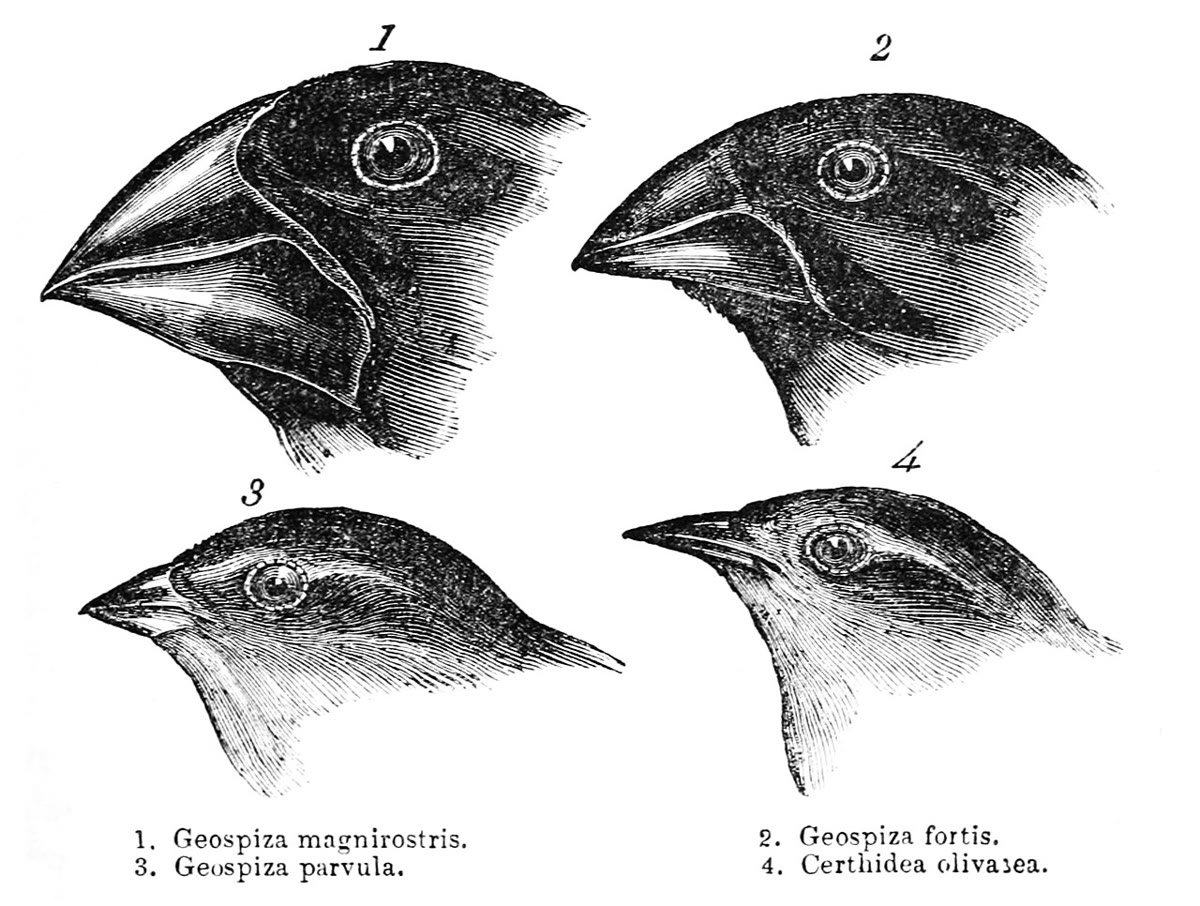
\includegraphics[width=0.44\linewidth]{images/book2/finches-gould.jpg}\hspace{0.04\linewidth}
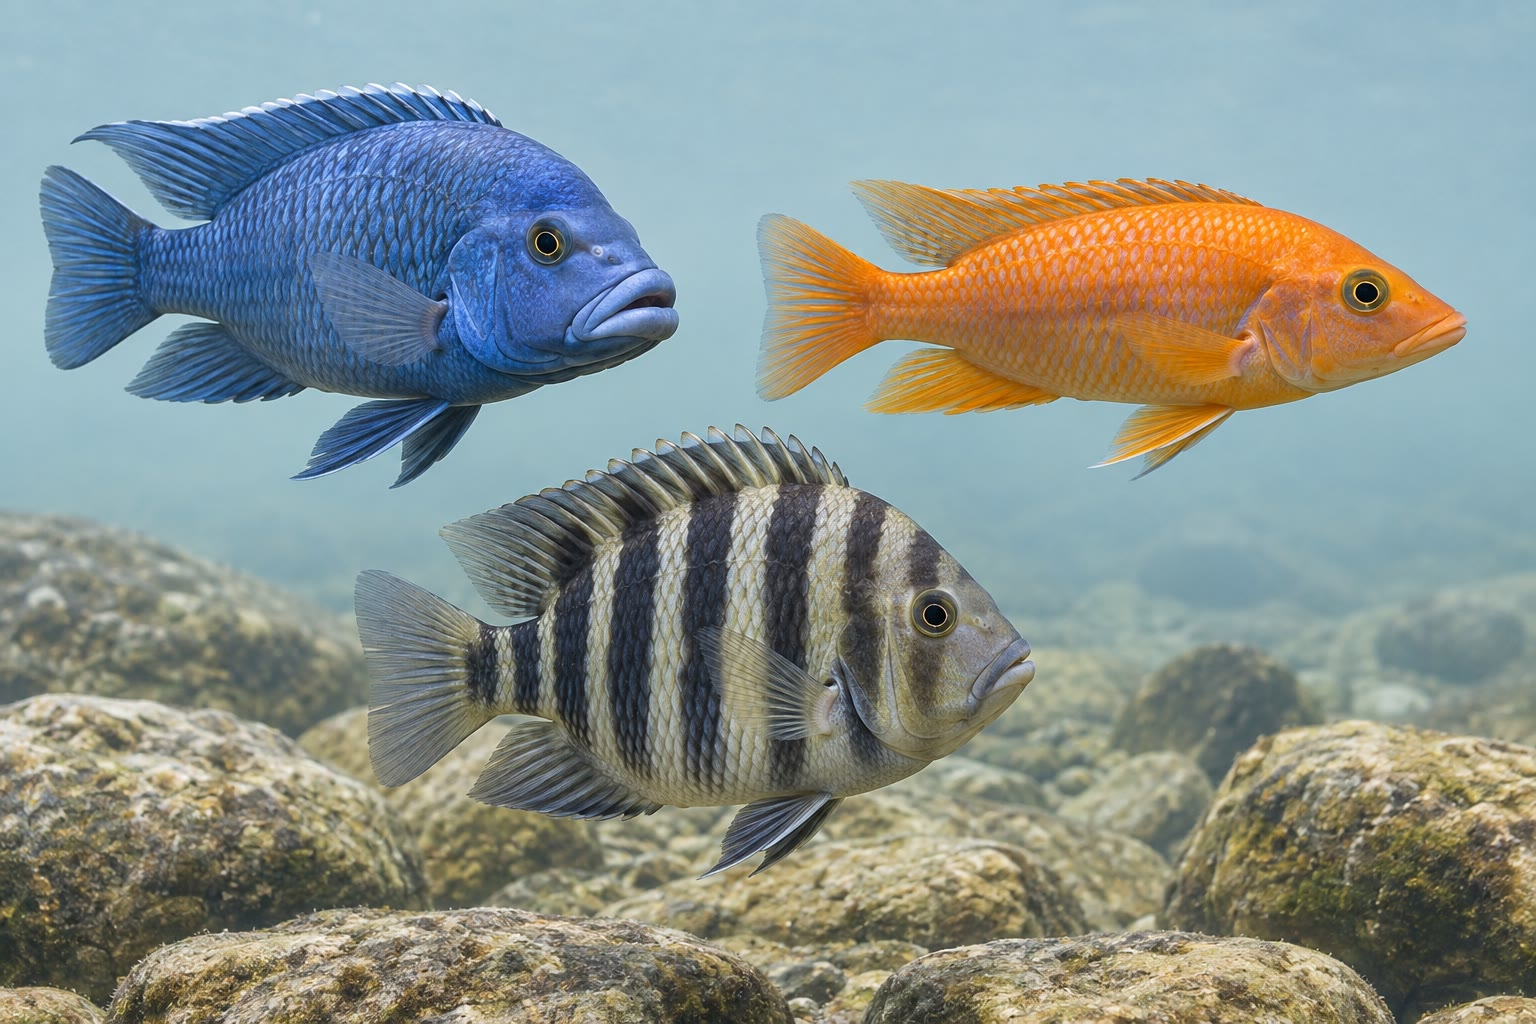
\includegraphics[width=0.44\linewidth]{images/book4/ai/b4-23-cichlids.jpg}

{\small Duas radiações. À esquerda: os tentilhões de Darwin desenhados
por Gould em 1845, um colono que se tornou muitos, distinguidos por seus
bicos. À direita: ciclídeos de um lago africano, centenas de espécies a
partir de alguns fundadores, cada uma com sua boca e sua dieta.}
\end{omfigure}

\section{Macroevolução: a visão de longo prazo}

\begin{proposition}[Ritmo e modo]\label{prop:b2:speciation:tempo}
\index{equilíbrio pontuado}\index{gradualismo}\index{extinção em massa}
Em algumas dezenas de gerações, a mariposa mudou de cor e o tentilhão,
de bico; em milhões de anos, o registro fóssil mostra linhagens que
quase não mudam durante longos períodos e depois, num instante geológico
de alguns milhares de anos, são substituídas por uma descendente
distinta --- o \emph{\omterm{prop:b2:speciation:tempo}{equilíbrio pontuado}}, que é o aspecto que tem a
\omterm{prop:b2:speciation:modes}{especiação alopátrica} em pequenas populações periféricas seguida de
sua expansão quando amostrada a cada cem mil anos; e mostra outras
linhagens, entre elas os cavalos, que mudam gradualmente ao longo de
dezenas de espécies. Acima da espécie, o registro é de renovação: a
maioria das espécies dura de um a dez milhões de anos, a taxa de
\emph{extinção de fundo} é de cerca de uma espécie em um milhão por ano
e, cinco vezes --- no fim do Ordoviciano, do Devoniano, do Permiano
(quando nove décimos das espécies marinhas desapareceram), do Triássico
e do Cretáceo ---, uma \emph{\omterm{prop:b2:speciation:tempo}{extinção em massa}} eliminou a maior parte
do que vivia em algumas centenas de milhares de anos e reiniciou o jogo,
com os sobreviventes se irradiando para os nichos esvaziados: os
mamíferos para o mundo dos dinossauros após o asteroide de 66 milhões de
anos atrás. A macroevolução é o padrão que a microevolução deste
capítulo e do anterior, prolongada por muito tempo e interrompida por
catástrofes, desenhou.
\end{proposition}

\begin{example}[Taxas comparadas]\label{ex:b2:speciation:rates}
A seleção sobre os tentilhões mudou a profundidade do bico em
\qty{4}{\%} em uma geração; toda a radiação das Galápagos, catorze
espécies a partir de um fundador, levou dois milhões de anos; a diferença
de tamanho corporal entre um camundongo e um elefante, cerca de $10^{5}$,
poderia ser produzida por uma seleção da intensidade da dos tentilhões
em algumas centenas de gerações --- e o registro mostra que levou
quarenta milhões de anos. O paradoxo se resolve notando que a seleção
raramente empurra no mesmo sentido por muito tempo: ela se inverte com o
clima, como aconteceu em Daphne Major no ano seguinte à seca, e a
\omterm{prop:b2:population-genetics:kinds}{seleção estabilizadora} mantém a maioria das linhagens onde estão. A
mudança sustentada é rara, e é por isso que a especiação, que precisa
dela, é lenta --- e por isso que, quando o mundo muda depressa, como no
\cref{ch:b2:global-change}, as linhagens que não conseguem acompanhar se
perdem.
\end{example}

\section{Exercícios}

\begin{exercise}[$\star$]\label{exo:b2:speciation:1}
Enuncie o \omterm{def:b2:speciation:species}{conceito biológico de espécie} e dê três casos em que ele não
pode ser aplicado, com o conceito usado em seu lugar.
\end{exercise}

\begin{exercise}[$\star$]\label{exo:b2:speciation:2}
Classifique como pré-zigótico ou pós-zigótico: duas rãs que se
reproduzem em meses diferentes; uma mula; um espermatozoide de ouriço-do-mar
que não consegue se ligar ao óvulo de outra espécie; plantas híbridas
vigorosas, mas cujas \omterm{def:b2:angiosperm-reproduction:seed}{sementes} não germinam; dois grilos de cantos
diferentes.
\end{exercise}

\begin{exercise}[$\star$]\label{exo:b2:speciation:3}
Defina \omterm{prop:b2:speciation:modes}{especiação alopátrica}, peripátrica, simpátrica e parapátrica,
com um exemplo de cada.
\end{exercise}

\begin{exercise}[$\star$]\label{exo:b2:speciation:4}
Enuncie os quatro desfechos da \omterm{thm:b2:speciation:lv}{competição de Lotka--Volterra} e a
condição de coexistência estável, em palavras.
\end{exercise}

\begin{exercise}[$\star\star$]\label{exo:b2:speciation:5}
Com $K_1 = 1000$, $K_2 = 800$, $\alpha = 0.5$, $\beta = 0.6$,
calcule as densidades de equilíbrio e verifique que cada espécie pode
invadir a capacidade de suporte da outra.
\end{exercise}

\begin{exercise}[$\star\star$]\label{exo:b2:speciation:6}
Com $K_1 = 1000$, $K_2 = 800$, $\alpha = 1.5$, $\beta = 0.3$, qual
espécie vence, e por quê? E se $\alpha = 1.5$ e $\beta = 1.5$?
\end{exercise}

\begin{exercise}[$\star\star$]\label{exo:b2:speciation:7}
Um tetraploide surge numa população \omterm{def:b2:meiosis-heredity:meiosis}{diploide}. Dê o número de
cromossomos de seus gametas, de um cruzamento com o \omterm{def:b2:meiosis-heredity:meiosis}{diploide} e dos
gametas desse híbrido, e explique por que o tetraploide fica isolado de
imediato. Por que, apesar disso, ele em geral não consegue persistir?
\end{exercise}

\begin{exercise}[$\star\star$]\label{exo:b2:speciation:8}
Duas populações fixaram, cada uma, 10 substituições desde que se
separaram, e cada par de novos \omterm{def:b2:meiosis-heredity:vocabulary}{alelos} dos dois lados é incompatível com
probabilidade $0.01$. Calcule o número esperado de incompatibilidades
agora e após 30 substituições em cada uma. O que isso prevê para a
relação entre o isolamento e o tempo?
\end{exercise}

\begin{exercise}[$\star\star$]\label{exo:b2:speciation:9}
Calcule a largura de uma \omterm{prop:b2:speciation:reinforcement}{zona híbrida} para uma dispersão $\sigma =
\qty{2}{km}$ por geração e uma desvantagem dos híbridos $s = 0.05$, e
para $\sigma = \qty{0.3}{km}$ e $s = 0.4$. Qual zona tem mais
probabilidade de terminar em reforço, e por quê?
\end{exercise}

\begin{exercise}[$\star\star\star$]\label{exo:b2:speciation:10}
Duas espécies de tentilhões competem por \omterm{def:b2:angiosperm-reproduction:seed}{sementes} com $\alpha = \beta = 0.9$ e
$K_1 = K_2 = 500$. Elas coexistem? O \omterm{prop:b2:speciation:displacement}{deslocamento de caracteres} reduz
$\alpha$ e $\beta$ a $0.4$: recalcule o equilíbrio. Explique, em
termos das isóclinas, o que o deslocamento fez.
\end{exercise}

\begin{exercise}[$\star\star\star$]\label{exo:b2:speciation:11}
Os Grant constataram que, após a seca de 2004, a profundidade média do
bico do tentilhão-terrestre-médio caiu \qty{0.7}{mm} com $h^{2} = 0.7$,
tendo os sobreviventes bicos \qty{1}{mm} menores que os da
população. Verifique a resposta com a \omterm{thm:b2:population-genetics:heritability}{equação do melhorista} e
explique por que a presença do tentilhão-terrestre-grande, e não apenas
a seca, determinou o sentido da mudança.
\end{exercise}

\begin{exercise}[$\star\star\star$]\label{exo:b2:speciation:12}
``As espécies são feitas por acidente e mantidas pela seleção.''
Discuta, com o modelo de dois lócus, o reforço e o papel da geografia.
\end{exercise}

\section{Problema: Dois tentilhões numa ilha}

\begin{problem}[{Problema de fim de semana --- um tentilhão residente
encontra um invasor: sua competição analisada no plano de fase, o
deslocamento do bico do residente previsto pela equação do melhorista e
o isolamento entre eles medido em relação a uma zona híbrida,
terminando com as densidades de equilíbrio, o deslocamento do bico e a
largura da clina}]
\label{pb:b2:speciation:1}
Espécie residente 1: $K_1 = 1200$, $r_1 = 0.5$ por ano; espécie
invasora 2: $K_2 = 400$. Antes do deslocamento, $\alpha = 0.9$, $\beta =
0.3$; uma seca reduz à metade as duas capacidades de suporte durante um
ano. Profundidade do bico da espécie 1: média de \qty{9.5}{mm},
desvio-padrão de \qty{0.8}{mm}, $h^{2} = 0.7$. Parâmetros da \omterm{prop:b2:speciation:reinforcement}{zona
híbrida}: $\sigma =
\qty{0.5}{km}$, $s = 0.2$.

\medskip
\noindent\textbf{Parte I --- A invasão.}
\begin{enumerate}
  \item Escreva as duas isóclinas e seus interceptos.
  \item A espécie 2 pode invadir a espécie 1 em $K_1$? A espécie 1
        pode invadir a espécie 2 em $K_2$? Conclua sobre o desfecho.
  \item Calcule as densidades de equilíbrio.
  \item Calcule $\mathrm{d}N_1/\mathrm{d}t$ no momento em que a espécie 2
        chega, com $N_2 = 20$ e $N_1 = 1200$. O que significa seu
        sinal?
  \item Durante a seca, os dois $K$ se reduzem à metade. Recalcule o
        equilíbrio e diga o que acontece com os efetivos de cada espécie.
  \item Por que o efeito do invasor sobre o residente ($\alpha = 0.9$)
        é maior que o do residente sobre o invasor ($\beta = 0.3$)?
\end{enumerate}

\medskip
\noindent\textbf{Parte II --- O deslocamento.}
Na seca, os indivíduos residentes de bico maior são os que mais competem
com o invasor e morrem: os sobreviventes têm um bico médio de
\qty{9.0}{mm}.
\begin{enumerate}[resume]
  \item Calcule o diferencial de seleção e a resposta.
  \item Dê o bico médio da geração seguinte.
  \item Após o deslocamento, $\alpha$ cai para $0.5$. Recalcule o
        equilíbrio (com os $K$ originais).
  \item Explique o que o deslocamento fez com a isóclina da espécie 1.
  \item Se uma seleção dessa intensidade agisse todos os anos, quantos
        anos levaria para deslocar o bico em \qty{2}{mm}? Por que
        isso não acontece?
  \item Compare com os dois milhões de anos de idade da radiação e
        comente.
\end{enumerate}

\medskip
\noindent\textbf{Parte III --- O isolamento.}
As duas espécies podem hibridizar; os híbridos têm bicos intermediários e
\omterm{def:b2:population-genetics:fitness}{aptidão} $1 - s$.
\begin{enumerate}[resume]
  \item Nomeie a barreira pré-zigótica que mantém a hibridização rara
        nos tentilhões de Darwin e um custo pós-zigótico dos
        híbridos.
  \item Calcule a largura de uma \omterm{prop:b2:speciation:reinforcement}{zona híbrida} entre eles para $\sigma
        = \qty{0.5}{km}$, $s = 0.2$.
  \item A ilha tem \qty{1}{km} de diâmetro. O que isso implica?
  \item Explique como o reforço procederia e sobre que caráter
        ele agiria.
  \item Duas populações do residente em ilhas diferentes fixaram, cada
        uma, 15 substituições desde que se separaram; os pares são
        incompatíveis com probabilidade $0.005$. Calcule o número esperado
        de incompatibilidades e diga se elas são espécies.
  \item O \omterm{def:b2:speciation:species}{conceito biológico de espécie}, o conceito morfológico e o
        conceito filogenético concordariam sobre as duas populações
        insulares? Explique.
\end{enumerate}

\medskip
\noindent\textbf{Parte IV --- A visão de longo prazo.}
\begin{enumerate}[resume]
  \item Se uma espécie dura em média 5 milhões de anos, qual é a taxa
        de extinção de fundo por espécie por ano? Para uma
        biota de 10 milhões de espécies, quantas extinções por ano?
  \item A taxa de extinção atual é estimada em 100 a 1000
        vezes a taxa de fundo. Quantas espécies por ano isso representa?
  \item Uma \omterm{prop:b2:speciation:tempo}{extinção em massa} elimina \qty{75}{\%} das espécies em
        \num{100000} anos. Compare sua taxa com a atual.
  \item Explique numa frase por que os sobreviventes de uma \omterm{prop:b2:speciation:tempo}{extinção em
        massa} se irradiam.
  \item Uma linhagem no registro muda pouco durante 3 milhões de anos e
        depois é substituída, em \num{20000} anos, por uma descendente
        distinta. Nomeie o padrão e dê o modo de especiação que o
        produz.
  \item Usando os \qty{4}{\%} por geração do tentilhão, quantas
        gerações de seleção sustentada dobrariam a profundidade do bico?
        Por que o registro fóssil mostra tais mudanças levando milhões
        de anos?
  \item Enuncie o resultado: o desfecho e o equilíbrio da competição
        antes e depois do deslocamento, o deslocamento do bico em uma
        geração e a largura da \omterm{prop:b2:speciation:reinforcement}{zona híbrida}.
\end{enumerate}
\end{problem}
